\documentclass[serif]{beamer}  

%compress

% Goettingen / Berkeley / Hannover / Singapore / Warsaw
\usetheme{Berlin}
\usecolortheme{beaver}

\usepackage[utf8x]{inputenc}	% Código fuente utf8
\usepackage{verbatim}
\usepackage{framed}				% marcos para texto
\usepackage{color}              % colores para el texto
\usepackage{graphicx}           % para poner im\'agenes



%TODO hacer anotaciones ;)

%%%%%%%%%%%%%%%%%%%%%%%%%%%%%%%%%%%%%%%%%%%%%%%%%%%%%%%%%%%%%%

\title[Falluto2.0] % (optional, only for long titles)
{Falluto2.0.}
%\subtitle{ Un model checker para sistemas tolerantes a fallas}
\subtitle{ UN MODEL CHECKER PARA SISTEMAS TOLERANTES A FALLAS}
\author[Monti] % (optional, for multiple authors)
{Raúl~E.~Monti \and Pedro~R.~D'Argenio}
\institute[FaMAF - UNC] % (optional)
{
Facultad de Matem\'atica, Astronom\'ia y F\'isica, Universidad Nacional de 
Córdoba
}
\date[4-2-2013] % (optional)
{Córdoba, Argentina. 2013}
\subject{Trabajo final de grado}

%%%%%%%%%%%%%%%%%%%%%%%%%%%%%%%%%%%%%%%%%%%%%%%%%%%%%%%%%%%%%%
%\AtBeginSection[]
%{
%  \begin{frame}
%    \frametitle{Tabla de contenidos}
%    \tableofcontents[currentsection]
%  \end{frame}
%}

%%%%%%%%%%%%%%%%%%%%%%%%%%%%%%%%%%%%%%%%%%%%%%%%%%%%%%%%%%%%%%

\begin{document}

%-------------------------------------------------------------
\frame{\titlepage}
%-------------------------------------------------------------

%-------------------------------------------------------------
\frame{\frametitle{Tabla de contenidos}\tableofcontents}
%-------------------------------------------------------------

%-------------------------------------------------------------
\section[Intro]{Introducción}
%%_____________________________________________________________
%\begin{frame}
%\frametitle{Sistemas tolerantes a fallas}
%\begin{itemize}\itemsep15pt
%\item Sistemas críticos.
%\item Fallas != Errores.
%\item Sistemas tolerantes a fallas.
%\item Model checking.
%\end{itemize}
%\end{frame}
%%_____________________________________________________________


%_____________________________________________________________
\begin{frame}
\begin{itemize}\itemsep15pt
\item {\Large \bfseries Sistemas críticos.}\\[5pt]
\hspace{0.5cm}Ejemplos: aviónica, equipos médicos, etc...
\item {\Large \bfseries Fallas (Fault) != Errores (Failure)}\\[5pt]
\hspace{0.5cm}\textbf{Falla} = cambio de estado que ``desestabiliza'' al sistema.\\[5pt]
\hspace{0.5cm}\textbf{Error} = desviación del comportamiento esperado.
\item {\Large \bfseries Sistemas tolerantes a fallas.}\\[5pt]
\hspace{0.5cm}No podemos evitar las fallas $\longrightarrow$ las superamos.
\end{itemize}
\end{frame}
%_____________________________________________________________


%_____________________________________________________________
\begin{frame}
{\Large \bfseries Model Checking.}
\begin{itemize}\itemsep15pt
\item Método formal para la verificación de propiedades sobre sistemas.
\item Exhaustivo sobre el espacio de estados del modelo finito.
\item NuSMV es un model checker basado en BDD.
\end{itemize}
\end{frame}
%_____________________________________________________________


%_____________________________________________________________
\begin{frame}[fragile]
\frametitle{Motivación}
{\fontsize{9pt}{13pt}\selectfont
\begin{minipage}{0.5\textwidth}
\begin{verbatim}
int file1 = 0, file2 = 0;

proctype process_1()
   bool on = false;
   while true:
      if on:
         if file1 == file2:
            synchronize();
            file1 = (file1+1)%10;
            send1();
         else:
            file1 = 0;
      else:
         on = true;
\end{verbatim}
\end{minipage}
\begin{minipage}{0.48\textwidth}
\begin{verbatim}



proctype process_2()
   bool on = false;
   while true:
      if on:
         if file1 == file2:
            synchronize();
            file2 = (file2+1)%10;
            send2();
         else:
            file2 = 0;
      else:
         on = true;
\end{verbatim}
\end{minipage}
} % end font size
\end{frame}
%_____________________________________________________________

%_____________________________________________________________
\begin{frame}
\frametitle{Objetivos}
\begin{itemize}\itemsep15pt
\item Continuar con el trabajo hecho en Falluto(Hames) y Offbeat(Bordenabe). 
\item Definir un lenguaje práctico para el modelado y verificación de 
sistemas tolerantes a fallas, que oculte las funcionalidad de las 
fallas y provea facilidades para la especificación de propiedades.
\item Elaborar un front-end para \textbf{NuSMV} que use este lenguaje.
\end{itemize}
\end{frame}
%_____________________________________________________________


%-------------------------------------------------------------


\section[Teoría]{Sistemas de transición de estados}

%_____________________________________________________________
\begin{frame}
\frametitle{Estructuras de Kripke}
Una estructura de Kripke sobre AP se define
como una 4-upla M = (S, I, R, L) donde\\[0.5cm]
\begin{itemize}
\item S es un conjunto finito de estados
\item I ⊆ S estados iniciales
\item R ⊆ S × S relación de transición left-total.
\item L: S → P(AP) función de etiquetado o
interpretación.
\end{itemize}
\end{frame}
%_____________________________________________________________

%_____________________________________________________________
\begin{frame}

En model checking usualmente sucede que:\\[0.5cm]
\begin{itemize}
\item $S$ es un conjunto de valuaciones sobre las variables del sistema.
\item $AP$ es un conjunto de expresiones booleanas sobre las variables.
\item $L(v) = \lbrace a \in AP~|~v(a)$ es verdadero$\rbrace$ con $v \in S$
\item $R$ explica la relación entre la valuación actual y la próxima
\end{itemize}

\end{frame}
%_____________________________________________________________


%_____________________________________________________________
\begin{frame}
\frametitle{Ejemplo de estructura de Kripke}
\begin{figure}
  \centering
    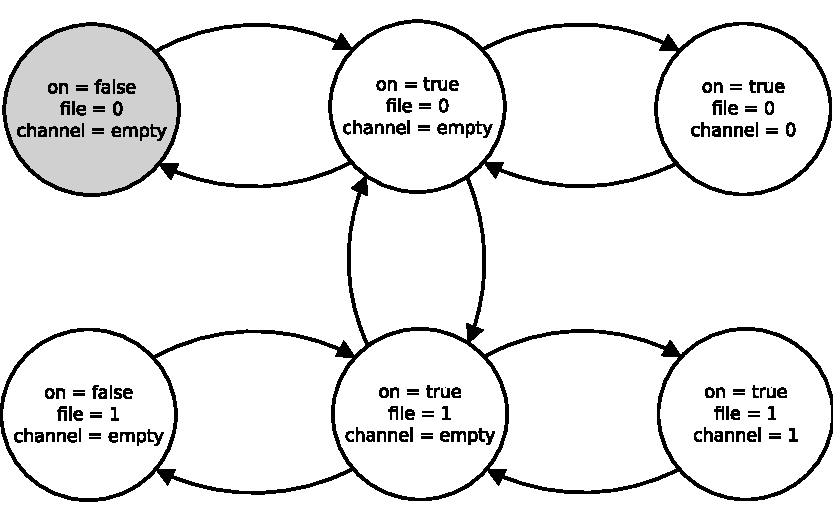
\includegraphics[scale=0.65]{imagenes/kripke.pdf}
\end{figure}
\end{frame}
%_____________________________________________________________


%_____________________________________________________________
\begin{frame}
\frametitle{LTS}
Un LTS es una 4-upla $M = (S,S_{0},L,R)$ donde:\\[0.3cm]
\begin{itemize}\itemsep10pt
\item $S$ es un conjunto de estados
\item $S_0 \subseteq S$ es un conjunto de estados iniciales
\item $L$ es un conjunto de etiquetas (nombres de transiciones)
\item $R \subseteq S \times L \times S$ es una relación ternaria de transiciones 
etiquetadas
\end{itemize}
~\\
Si $s1, s2 \in S$, $l \in L$, y $(s1,l,s2) \in R$, entonces existe una 
transición con nombre $l$ desde el estado $s1$ al estado $s2$.
\end{frame}
%_____________________________________________________________


%_____________________________________________________________
\begin{frame}
\frametitle{Ejemplo de LTS}
\begin{figure}
  \centering
    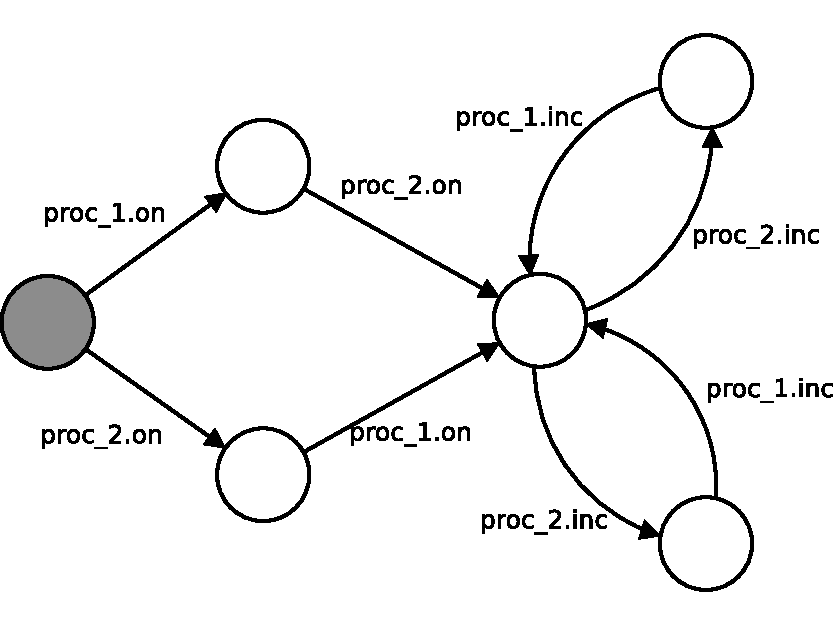
\includegraphics[scale=0.65]{imagenes/lts.pdf}
\end{figure}
\end{frame}
%_____________________________________________________________


%-------------------------------------------------------------


\section[Lenguaje]{Lenguaje de Falluto2.0}


%_____________________________________________________________
\begin{frame}[fragile]
\frametitle{El lenguaje de NuSMV}

{\fontsize{8pt}{10pt}\selectfont
\begin{minipage}{0.5\textwidth}
{\large \bfseries Modelado}
\begin{framed} \begin{verbatim}
MODULE main()
  VAR
    v1:boolean;
    v2:{1,2,a,b};

  INIT
    v1 & v2 = a

  TRANS
    ( v1 -> next(v2) in {a,b}
    & !v1 -> next(v2) in {1,2}
    ) 
    | next(v1) = !v1
\end{verbatim}
\end{framed}
\end{minipage}
\hspace{0.04\textwidth}
\begin{minipage}{0.44\textwidth}
{\large \bfseries Propiedades}
\begin{framed}
\begin{verbatim}
LTLSPEC G v1 = FALSE

CTLSPEC AG TRUE
\end{verbatim}
\end{framed}
{\large \bfseries Fairness}
\begin{framed}
\begin{verbatim}
FAIRNESS v2 in {1,a}

COMPASSION (v2 = 1 , !v1)
\end{verbatim}
\end{framed}
\end{minipage}
} %end fontsize
\end{frame}
%_____________________________________________________________


%_____________________________________________________________
\begin{frame}[fragile]
\frametitle{El lenguaje de Falluto2.0}
{\fontsize{8pt}{10pt}\selectfont
\begin{minipage}{0.5\textwidth}
{\large \bfseries Modelado}
\begin{framed} 
\begin{verbatim}
PROCTYPE proc( cxtv1, ctxv2 
             ; sync1, sync2)
  VAR
    var1 : bool
   
  INIT
    {formula}

  TRANS
    [name]: enable => changes
    [sync1] ...
    []: ...
ENDPROCTYPE
...
\end{verbatim}
\end{framed}
\end{minipage}
\hspace{0.04\textwidth}
\begin{minipage}{0.44\textwidth}
{\large \bfseries Instanciación, propiedades y fairness}
\begin{framed}
\begin{verbatim}
INSTANCE inst1 =
    proc(inst2.v,TRUE,s1,s1)

INSTANCE inst2 = proc2(s1)

LTLSPEC ...
CTLSPEC ...
NORMAL_BEHAIVIOUR ...

FAIRNESS ...
COMPASSION( ... )

\end{verbatim}
\end{framed}
\end{minipage}
} %end fontsize

\end{frame}
%_____________________________________________________________



%_____________________________________________________________
\begin{frame}
\frametitle{Descripción de transiciones}
\texttt{[nombre]: cond\_habilitación $=>$ post\_condición}\\[0.5cm]
La condición de habilitación es una fórmula
booleana sobre el estado actual del sistema.\\[0.5cm]
Las post condiciones son listas de next-
valores: $$v1' = f1,~v2' = f2,~v3' = f3,~...$$
\end{frame}
%_____________________________________________________________


%_____________________________________________________________
\begin{frame}
\frametitle{Inyección de fallas}
La inyección de fallas se realiza de modo declarativo, en la 
sección introducida por la palabra reservada \texttt{FAULT} de 
cada proctype:\\[0.5cm]
\texttt{nombre : cond\_habilitaci\'on => post\_condición is TYPE} \\[0.5cm]
donde \texttt{TYPE} puede ser: \\[0.5cm]
\begin{itemize}
\item \texttt{STOP[(trans1, trans2, ...)]}
\item \texttt{BYZ([var1, var2, ...])}
\item \texttt{TRANSIENT}
\end{itemize}
\end{frame}
%_____________________________________________________________


%_____________________________________________________________
\begin{frame}[fragile]
\frametitle{El lenguaje de Falluto2.0}
{\fontsize{7pt}{10pt}\selectfont
\begin{minipage}{0.45\textwidth}
{\large \bfseries Modelado}
\begin{framed} 
\begin{verbatim}
PROCTYPE machine(; send)
  VAR
    on : bool
    file : 0..9
  INIT
    !on & file = 0
  TRANS
    [send]: on 
            => 
            file' = (file+1)%10
    [OnOff]: => on' = !on
ENDPROCTYPE
\end{verbatim}
\end{framed}
\end{minipage}
\hspace{0.04\textwidth}
\begin{minipage}{0.45\textwidth}
{\large \bfseries Inyección de falla}
\begin{framed}
\begin{verbatim}
PROCTYPE machine(; transfer)
  VAR
    ...
\end{verbatim}
\texttt{\color{red}~~FAULT\\$~~~~~$
f1: is STOP(OnOff)\\$~~~~~$
f2: file = 9 => is\\$~~~~~~~~~~$ BYZ(file)\\$~~~~~$
f3: => file' = 0 is\\$~~~~~~~~~~$ TRANSIENT}
\begin{verbatim}
  INIT ...
  TRANS ...
ENDPROCTYPE
\end{verbatim}
\end{framed}
\end{minipage}
} %end fontsize

\end{frame}
%_____________________________________________________________


%_____________________________________________________________
\begin{frame}
\frametitle{Especificación de propiedades}
\textbf{Propiedades como en NuSMV:}\\[0.3cm]
\begin{center}\texttt{LTLSPEC q}

\texttt{CTLSPEC q}\end{center}
\textbf{Propiedades sobre escenarios comunes}\\[0.3cm]
``Si solo hago buenas transiciones entonces q es verdadera'':\\[0.2cm]
\begin{center} \texttt{NORMAL\_BEHAVIOUR -> q}\end{center}
``Si eventualmente las fallas dejan de ocurrir entonces q es
verdadera'':\\[0.2cm]
\begin{center} \texttt{FINITELY\_MANY\_FAULTS -> q}\end{center}
\end{frame}
%_____________________________________________________________


\section[Compilaci\'on]{Compilación de Falluto2.0}


%_____________________________________________________________
\begin{frame}
\frametitle{Compilación de transiciones}
\textbf{\Large Transiciones comunes:}\\[0.3cm]
\texttt{[trans]: pre => pos1, pos2, ...}\\[0.3cm]
Se compila como:
\begin{framed}
$act\#var'~=~trans~\wedge~!stop~\wedge~pre~\wedge~pos1~\wedge~pos2~\wedge...\wedge~unchanged$
\end{framed}
Donde:
$$unchanged = \bigwedge_{v\in V}(v' = v) \text{ con }V = Vars - POS - act\#var$$

\end{frame}
%_____________________________________________________________


%_____________________________________________________________
\begin{frame}
\frametitle{Compilación de transiciones}
\textbf{\Large Transiciones sincronizadas:}\\[0.3cm]
Por cada sincronizaci\'on tendremos:
\begin{framed}
$act\#var' = syncname~\wedge~!stop~\wedge~pre1~\wedge~pre2~\wedge~...$
$~\wedge~pos1~\wedge~pos2~\wedge~...~\wedge~unchanged$\\[0.3cm]
\end{framed}
Donde
$$unchanged = \bigwedge_{v \in V}(v' = v) \text{ con }V = Vars 
- \bigcup (pos_j) - act\#var$$
$stop$ involucra las fallas que afectan cada una de las 
transiciones sincronizadas.
\end{frame}
%_____________________________________________________________


%_____________________________________________________________
\begin{frame}
\frametitle{Compilación de transiciones}
\textbf{\Large Transiciones de falla:}\\[0.3cm]
\texttt{fault: pre => pos1, pos2, ... is Type}\\[0.3cm]
Compila a:
\begin{framed}
$act\#var' = fault~\wedge~!fault\_active~\wedge~pre~\wedge~fault\_active'$
$~\wedge~pos1~\wedge~pos2~\wedge~...~\wedge~unchanged$
\end{framed}
$!fault\_active$ y $fault\_active'$ solo en caso de fallas permanentes.
\end{frame}
%_____________________________________________________________


%_____________________________________________________________
\begin{frame}
\frametitle{Compilación de transiciones}
\textbf{\Large Transición de deadlock:}\\[0.3cm]
\begin{framed}
$act\#var' = dk\#trans~\wedge~neg\_pre~\wedge~unchanged$
\end{framed}
$neg\_pre~=~\bigwedge_{i \in instances}~\bigwedge_{t \in transN_i}~(~!~pre_{i,t}~|~Stop_{i,t}~)$\\[0.3cm]
$~~~~~~~~~~~~~~~~\bigwedge_{s \in sincro}~(~!~pre_s~|~Stop_s~)$\\[0.3cm]
Donde:\\[0.3cm]
$unchanged = \bigwedge_{v \in V}(v' = v) \text{ con } v \in Var - act\#var$
\end{frame}
%_____________________________________________________________

%_____________________________________________________________
\begin{frame}
\frametitle{Compilación de transiciones}
\textbf{\Large Verificación de deadlock}\\[0.3cm]
Usamos la propiedad \texttt{CHECK\_DEADLOCK}.\\[0.3cm]
Es compilada como:
\begin{framed}
$CTLSPEC~AG~act\#var~!=~dk\#trans$
\end{framed}
Notar relación con la transición de deadlock.
\end{frame}
%_____________________________________________________________



%_____________________________________________________________
\begin{frame}
\frametitle{Compilación de transiciones}
\textbf{\Large Compilación de la relación de transición final:}\\[0.3cm]
Consiste de la disyunción \textit{exclusiva} de cada una de las 
transiciones del sistema:
\begin{framed}
$$\bigvee_{t \in T} t $$
\end{framed}
Con $T =$ transiciones\_comunes $\bigcup$ transiciones\_sincronizadas 
$\bigcup$ transiciones\_de\_falla $\bigcup$ transición\_de\_deadlock
\end{frame}
%_____________________________________________________________

\section[Fairness]{Fairness en Falluto2.0}

%_____________________________________________________________
\begin{frame}
\frametitle{Weak fairness entre procesos}
\begin{framed}
$F~G~habilitada \rightarrow G~F~atendida$
\end{framed}
Compilación:
\begin{framed}
$FAIRNESS~(\bigvee_{t \in T_{N_i}} act\#var = t)~\vee~instanceDK$
\end{framed}
Donde $instanceDK = \bigwedge_{t \in T_i}~!~pre_t~$\\[0.5cm]
\texttt{INST\_WEAK\_FAIR\_DISABLE:}\\
deshabilita la condición de fairness entre los procesos.
\end{frame}
%_____________________________________________________________


%_____________________________________________________________
\begin{frame}
\frametitle{Fairness con respecto a fallas}
\begin{framed}
$G~F~transicion\_buena$
\end{framed}
Compilación:
\begin{framed}
$FAIRNESS~(\bigvee_{t \in {T_N}} act\#var = t)~\vee~act\#var = dk\#trans$
\end{framed}
\texttt{FAULT\_FAIR\_DISABLE:}\\
deshabilita la condición de que a menudo se haga una transición normal.\\[0.3cm]
\end{frame}
%_____________________________________________________________

\section[Trazas]{Interpretación de trazas}

%_____________________________________________________________
\begin{frame}[fragile]
\frametitle{Intérprete de trazas}
{\fontsize{9pt}{12pt}\selectfont
\begin{minipage}{0.5\textwidth}
\begin{verbatim}
-> State: 1.1 <-
action# = dk#action
lvar#inst#var1 = FALSE
lvar#inst#var2 = 0
ipc#inst = 0
-> State: 1.2 <-
action# = trans#inst#trans1
lvar#inst#var2 = 1
-> State: 1.3 <-
lvar#inst#var2 = 2
-> State: 1.4 <-
action# = trans#inst#trans2
lvar#inst#var1 = TRUE
ipc#inst = 1
\end{verbatim}
\end{minipage}
\hspace{0.04\textwidth}
\begin{minipage}{0.44\textwidth}
\begin{verbatim}
---> State: 0 <---
inst var1 = FALSE
inst var2 = 0

@ [action] inst / trans1
---> State: 1 <---
inst var2 = 1

@ [action] inst / trans1
---> State: 2 <---
inst var2 = 2

@ [action] inst / trans2
---> State: 3 <---
inst var1 = TRUE
\end{verbatim}
\end{minipage}
} %end fontsize
\end{frame}
%_____________________________________________________________


\section{Resultados}
%_____________________________________________________________
\begin{frame}
\frametitle{A favor}
\begin{itemize}\itemsep15pt

\item Lenguaje simple y declarativo para la verificación de sistemas tolerantes 
a fallas.

\item Herramienta que abstrae y automatiza la verificación de manera eficiente.

\item Efectividad comprobada en casos reales de verificación (sistema de 
comunicación inter-satelital).

\end{itemize}
\end{frame}
%_____________________________________________________________


%_____________________________________________________________
\begin{frame}
\frametitle{En contra}
\begin{itemize}\itemsep15pt
\item Soporta solo una pequeña porción de las capacidades de NuSMV.
\item Se debería ampliar la batería de meta-propiedades.
\item El lenguaje de modelado podría hacerse más práctico en ciertos aspectos.
\end{itemize}
\vspace{15pt}
\begin{center}{\LARGE ~}\end{center}
\end{frame}
%_____________________________________________________________


%_____________________________________________________________
\begin{frame}
\frametitle{En contra}
\begin{itemize}\itemsep15pt
\item Soporta solo una pequeña porción de las capacidades de NuSMV.
\item Se debería ampliar la batería de meta-propiedades.
\item El lenguaje de modelado podría hacerse más práctico en ciertos aspectos.
\end{itemize}
\vspace{15pt}
\begin{center}{\color{red} \LARGE En realidad es trabajo a futuro ;)}\end{center}
\end{frame}
%_____________________________________________________________



\section[Ejemplo]{Ejemplo de uso}
%_____________________________________________________________
\begin{frame}
\frametitle{Ejemplo}
\begin{center}{\LARGE \emph{Cómo usar Falluto2.0}}\end{center}
\end{frame}
%_____________________________________________________________




%_____________________________________________________________
\begin{frame}
\frametitle{Fin}
\begin{center}{\LARGE \emph{FIN}}\end{center}
\end{frame}
%_____________________________________________________________


%-------------------------------------------------------------


\end{document}
